\documentclass[12pt]{report}

\usepackage[brazil,american]{babel}
\usepackage[utf8]{inputenc}
\usepackage[a4paper, total={6.5in, 9.5in}]{geometry}

\usepackage{titlesec}
\titleformat{\chapter}[display]
  {\normalfont\bfseries}{}{0pt}{\Huge}

\usepackage{url}
\usepackage{graphicx}
\usepackage{authblk}
\usepackage{hyperref}
\usepackage{lipsum}
\usepackage{xcolor}
\usepackage{float}

% \pagecolor[rgb]{0.1,0.1,0.1}
% \color[rgb]{0.9,0.9,0.9}

\begin{titlepage}
    \title{
        
\includegraphics[width=4cm]{img/logo.jpg} \\ 
        \large
        Dep. Ciência da Computação -- Universidade de Brasília (UnB)\\
        CIC0207 - Projeto Interdisciplinar de Licenciatura em Computação \\
        \vfill 
        \vfill
        \LARGE
        \textbf{Portal de Equações Matemáticas de Primeiro e Segundo Grau}
    }

    \author{
        Letícia Dias Soares Alves, 18/0022059\\
        Pedro Henrique de Brito Agnes, 18/0026305
    }
    
    \affil{
        \vfill
        \vfill
        \vfill
        Professora \\
        Dr.a Letícia Lopes Leite
    }

    \date{Brasília\\Novembro de 2020}

\end{titlepage}

\begin{document}
\maketitle

\selectlanguage{american}
\begin{abstract}
  With the great difficulty that can be observed on math students on school, it's necessary that they have access to some tools meant to help on the understanding of the subject and even awake their interest on it. To solve the problem, the portal of first and second degree equations was developed with the goal to help the students on learning the so feared subject that is used on many others, taking advantage of the interdisciplinarity with physics and chemistry among others.

  The portal have an explanation of the subject, with videos, curiosities, among others. There is also a selection of exercises to help the students to practice what was learned, and also the resolution of each exercise so they can check their answers to see if its right or where they commit a mistake. At last, there is also a page that allows the student to type any equation to see the answer aswell as the graphic to the function that represents it, which can help on the understanding of the equations by itself when used along with the resources of the website.
\end{abstract}

\selectlanguage{brazil}
\begin{abstract}
  Com a grande dificuldade que pode ser observada nos estudantes em matérias de matemática, torna-se necessária a disponibilidade de ferramentas para o auxílio do ensino de forma melhorar o entendimento da matéria e até a despertar o interesse dos alunos. Para solucionar o problema, o portal de equações de primeiro e segundo grau foi desenvolvido com o objetivo de auxiliar os alunos no aprendizado desta matéria tão temida que é utilizada em diversas outras, tomando vantagem da interdisciplinaridade com a física, química e outros.

  O portal contém explicações do conteúdo de equações, com vídeos explicativos, curiosidades, entre outros. Também possui uma seleção de exercícios para ajudar os estudantes a praticar o conhecimento adquirido com a resolução disponível caso o usuário deseje conferir a resposta para ver se acertou ou onde cometeram um erro. Por fim, uma página que permite ao estudante digitar uma equação quealquer para obter a resposta para a mesma, assim como o gráfico da função que a representa, o que pode auxiliar no entendimento das equações em si, quando usado em conjunto com os materiais disponíveis no portal.
\end{abstract}

\tableofcontents
\newpage

\chapter{Introdução}
Na matemática entendemos equações como expressões algébricas que possuem incógnitas representadas por letras (notações mais usadas são: x,y,z,w), e foram criadas há muito tempo atrás para a solução de problemas quando o número é desconhecido. As equações de primeiro (onde o expoente da incógnita é igual a 1) e segundo grau  (onde o expoente da incógnita é igual a 2), desenvolvem um papel muito importante na rotina de alunos e professores, mas que muitas das vezes essas matérias acabam sendo passadas de forma tradicional e mecânica, que pode acabar interferindo na assimilação do conteúdo.

As equações são muito utilizadas no ensino fundamental (onde são ensinadas), caso o aluno não consiga assimilar a matéria, terá muitas dificuldades, pois, este mesmo conteúdo é usado no nível médio e superior. Esse trabalho é desenvolvido com a finalidade de mostrar uma forma alternativa de passar esses conteúdos utilizando ferramentas que mostrem outras formas de apresentar a mesma matéria. Nossa ideia foi desenvolver um software onde o aluno possa escrever a equação desejada e ver a resolução da questão mostrando o passo a passo. 

\chapter{Problema}
É comum atualmente muitos professores usarem metodologias tradicionais (onde o professor é o centro do processo de ensino aprendizagem), e isso acaba afetando todos os alunos que não conseguem se encaixar neste sistema. A tecnologia poderia auxiliar tanto os professores quanto os alunos, pois com o auxílio da tecnologia poderiam ser criadas muitas ferramentas para cada tipo de pessoa, alguns ferramentas com mais textos, imagens, vídeo aulas específicas, ou até mesmo jogos, questionários, etc.

A dificuldade na resolução de equações ao longo do período escolar é natural e se torna presente em muitos alunos, que acabam por perder todo o interesse pela matéria, em especial quando não conseguem encontrar uma aplicabilidade para elas. A baixa capacidade de resolução de equações pode afetar negativamente o desempenho em matérias como física, química e a própria matemática, em que este conteúdo é usado o tempo todo e qualquer pequeno erro já faz com que o aluno perca toda uma questão. O projeto tem como finalidade, a descomplicação do conteúdo por meio de um \textit{website}.

\chapter{Esboços das telas}
O software em desenvolvimento é, de certa forma inspirado no \href{https://pt.symbolab.com/}{Symbolab} e no Photomath que são "calculadoras" avançadas que mostram a resolução passo a passo dos exercícios desde os mais simples até os mais avançados com até matérias do ensino superior. O portal será composto de uma \textit{home}, uma página com a explicação do conteúdo e outra com o modo de calculadora para a resolução de exercícios.

\section{Página inicial}
A página principal do portal será bem simples, mostrando apenas uma introdução e detalhes sobre o projeto e um guia básico de utilização da aplicação, assim como links para as outras páginas. Também incluirá referências e informações dos autores como as de contato para que os estudantes possam conferir as fontes, assim como informar sobre erros na aplicação por e-mail, caso existam.

\begin{figure}[H]
    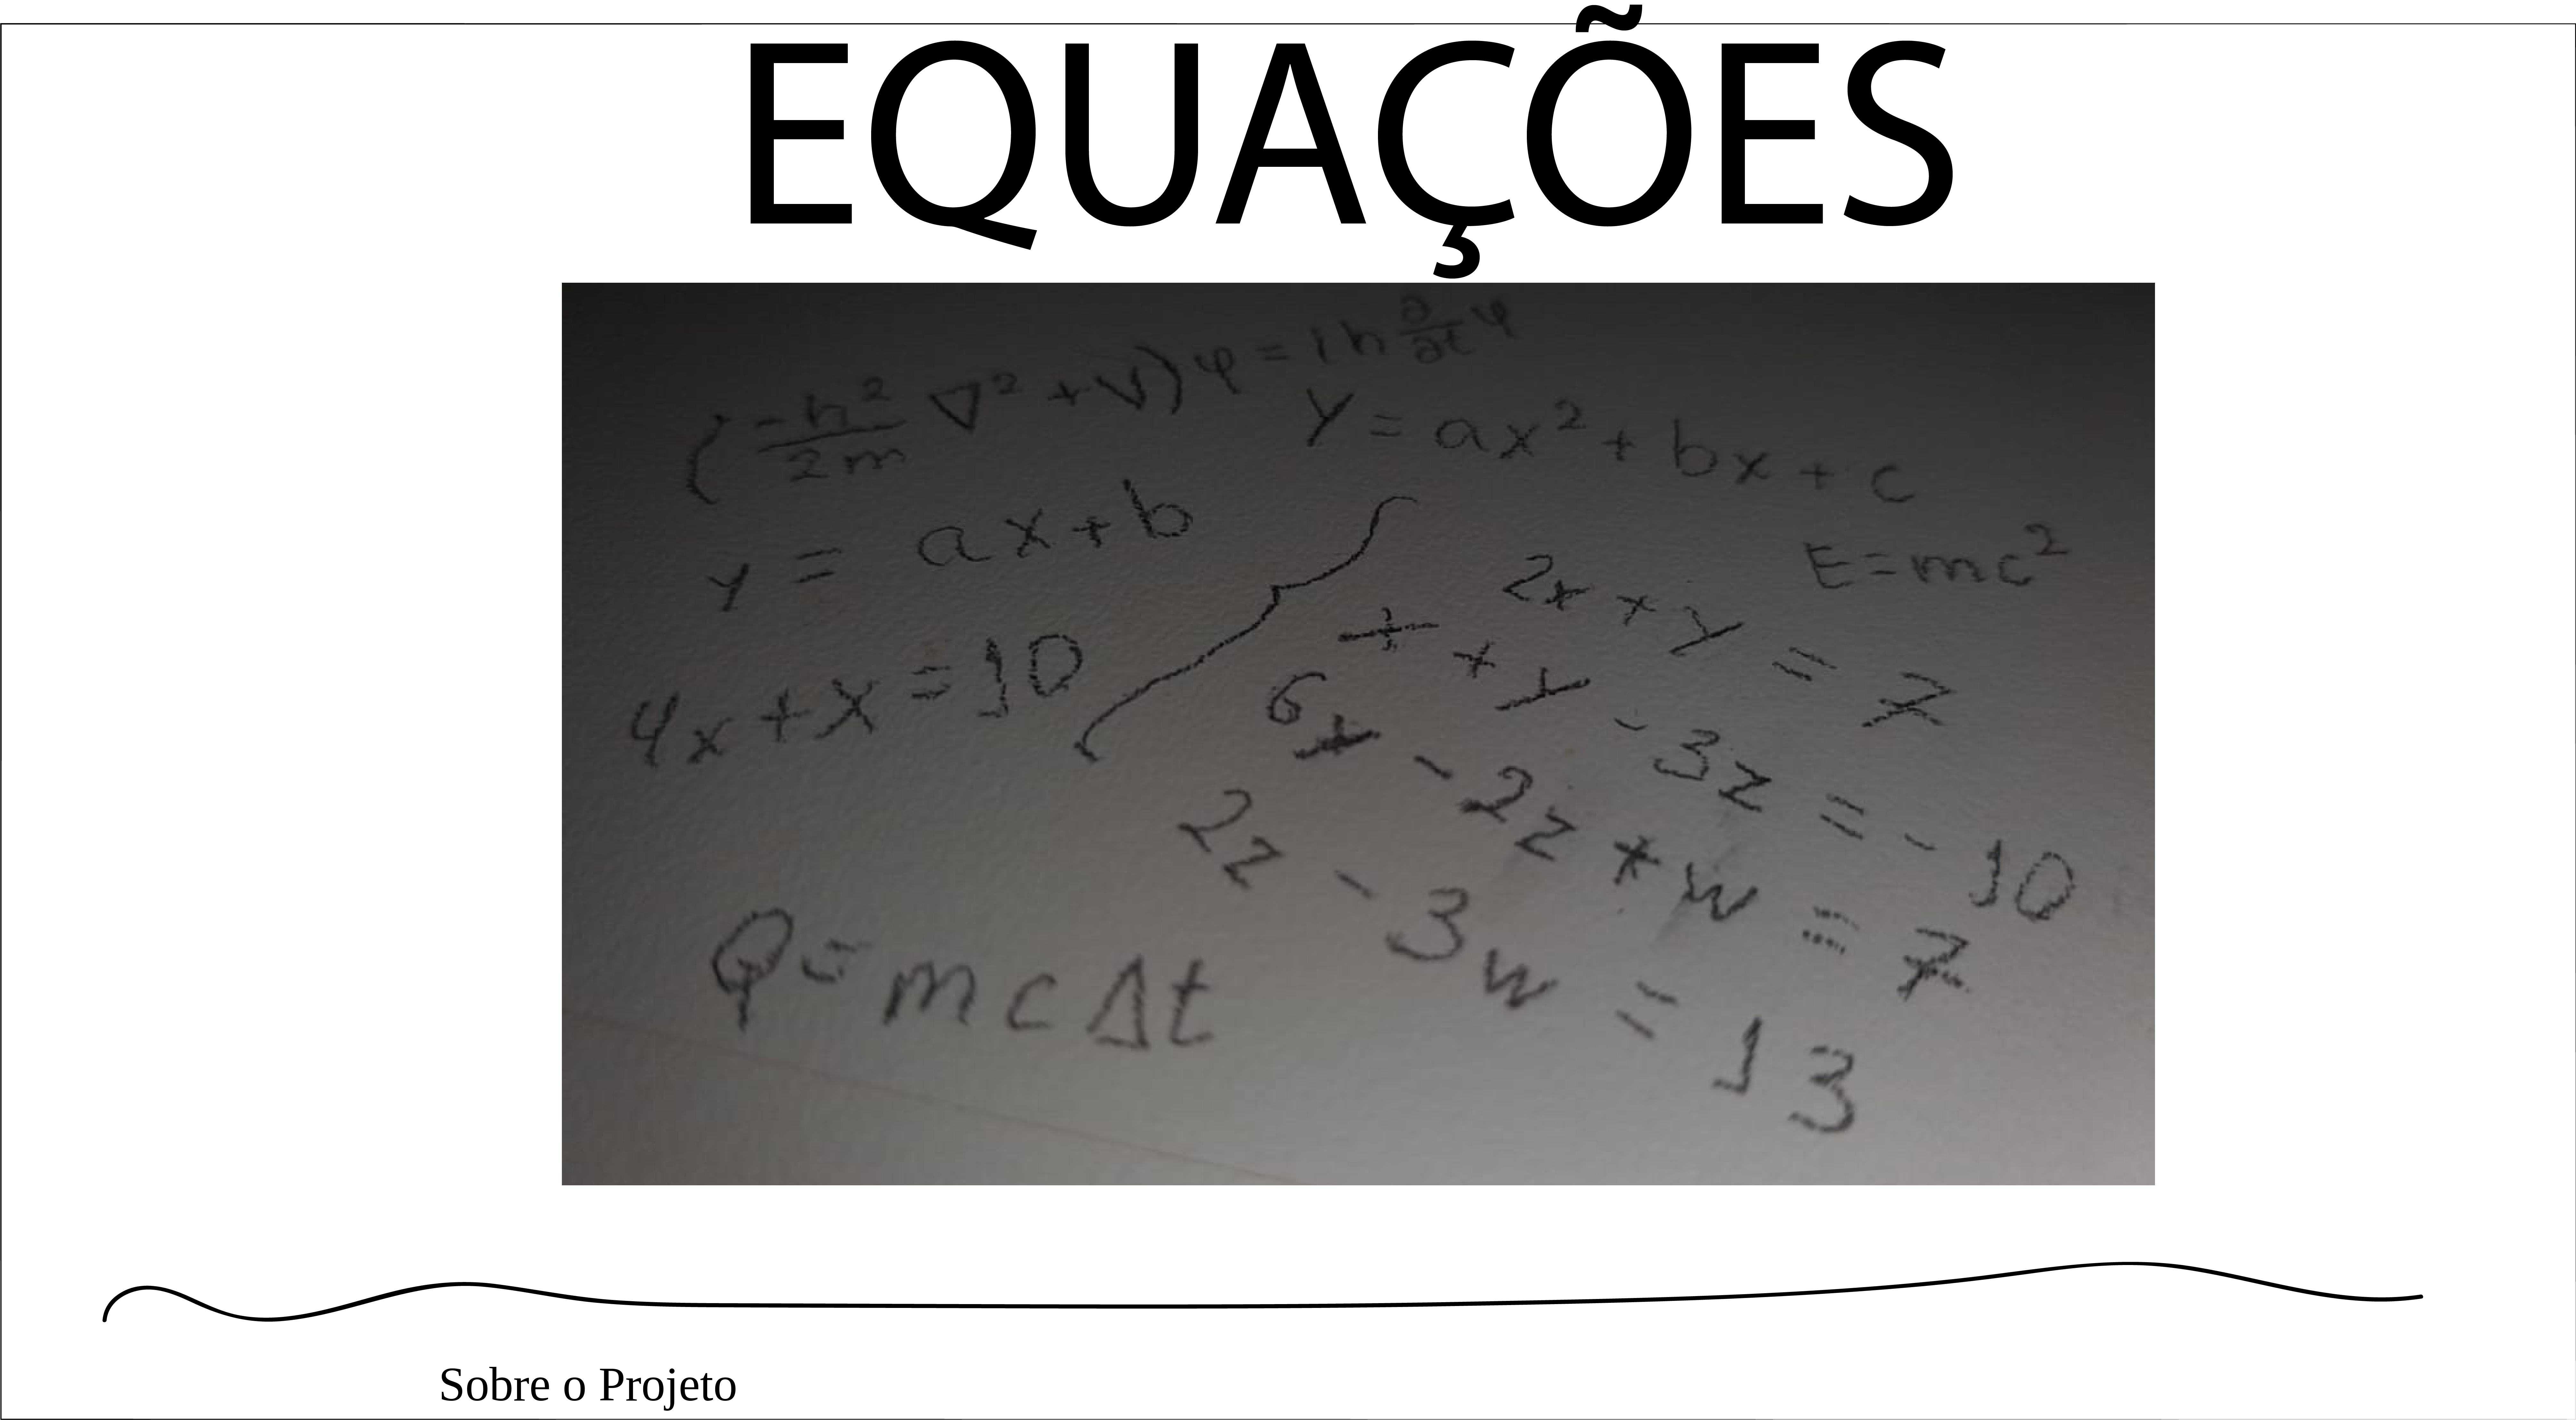
\includegraphics[width=1\textwidth]{img/c.png}
    \caption{Esboço da tela \textit{Home}}
\end{figure}

\section{Exercícios}
Uma segunda tela será a de exercícios e explicação do conteúdo e possuirá vídeos, gráficos, exemplos de problemas resolvidos com a opção de clicar em cima para mostrar o passo a passo da resolução da equação se o usuário quiser tentar resolver antes por si só, entre outros para a explicação do conteúdo. O portal é planejado para possuir também um "dark mode" para agradar a todo tipo de público que poderá ser ativado/desativado pelo botão na barra de navegação, porém não está no esboço e apenas atera a aparência do portal sem mudar as posições de nenhum elemento, apenas alterando o esquema de cores para mais escuros.

\begin{figure}[H]
    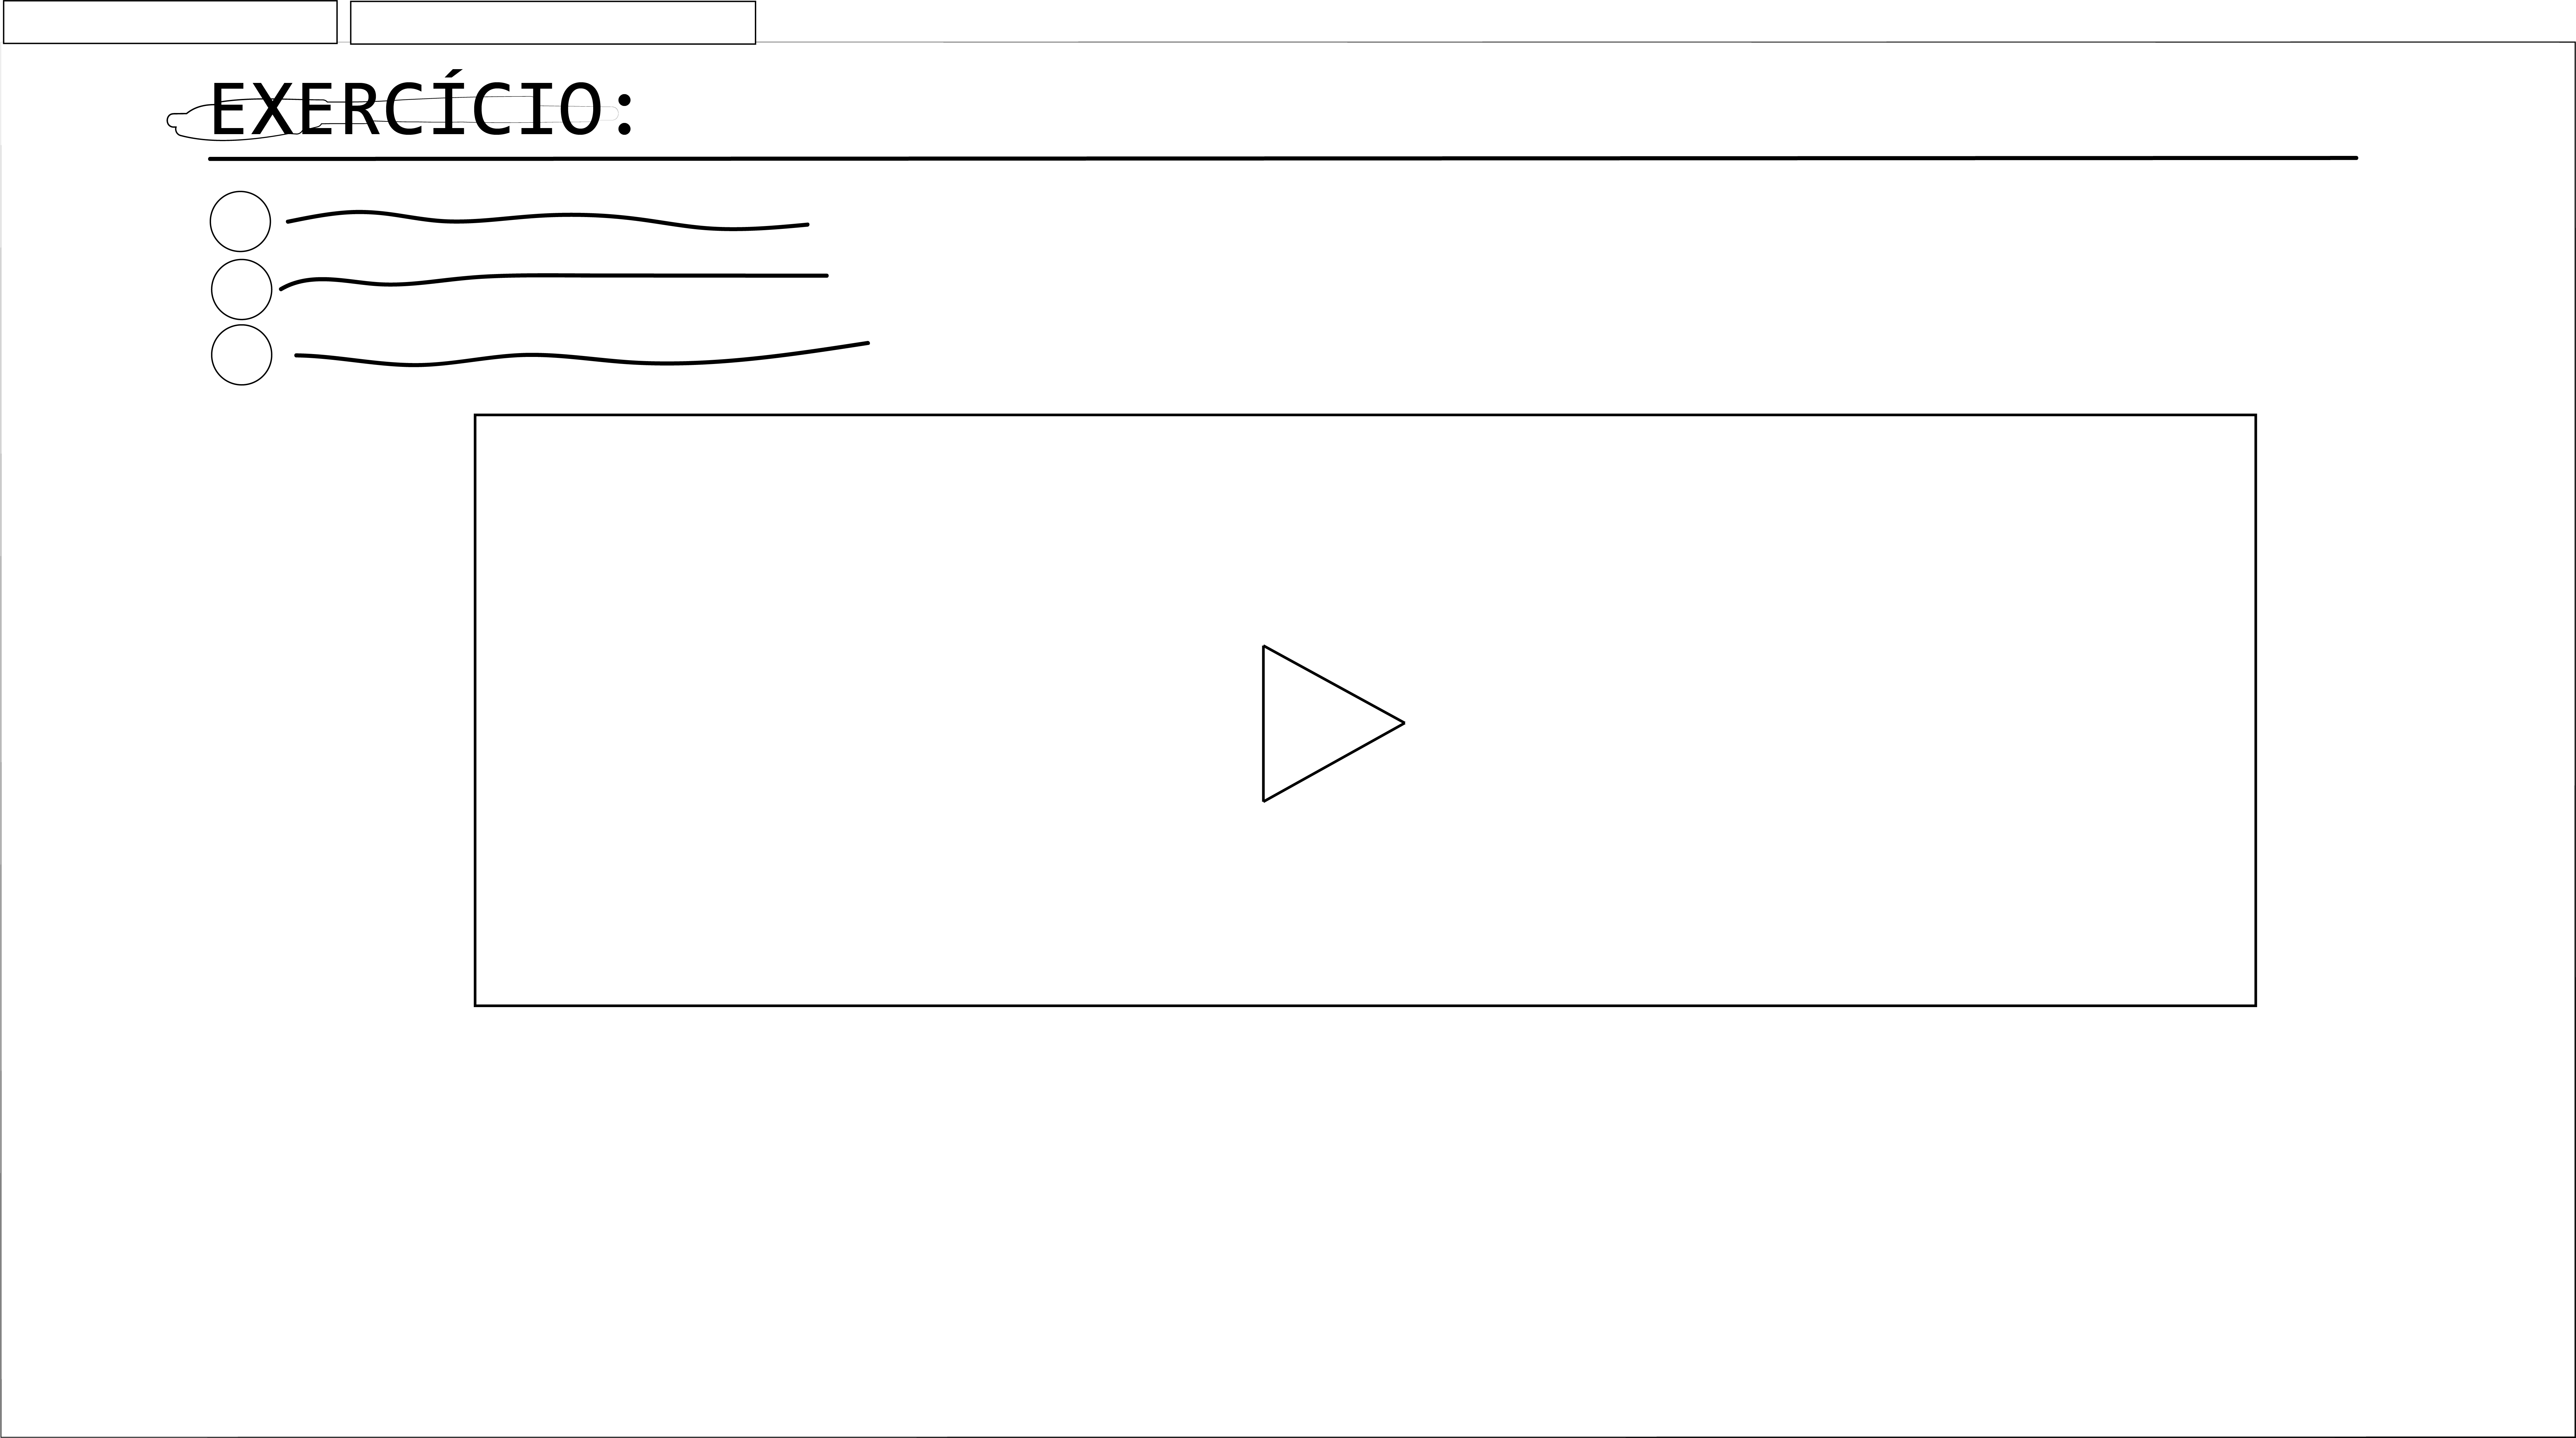
\includegraphics[width=1\textwidth]{img/A.jpg}
    \caption{Esboço da tela de exercícios}
\end{figure}

Podemos ver um projeto de uma barra de navegação que manterá os links para outras páginas mais acessível, assim como incluir outras opções importantes também, como a opção do modo escuro.

\section{Modo interativo}
Por fim, teremos a última página que poderá ser acessada por um link disponível na barra de navegação e vai conter a seção de fazer os exercícios informados pelo usuário. A tela consistirá basicamente de um "input" de texto onde será informada uma equação e abaixo será mostrada a resposta ao clicar em um botão. É planejado de ser mostrado também o gráfico da equação que for informada para melhor visualização e entendimento.

\begin{figure}[H]
    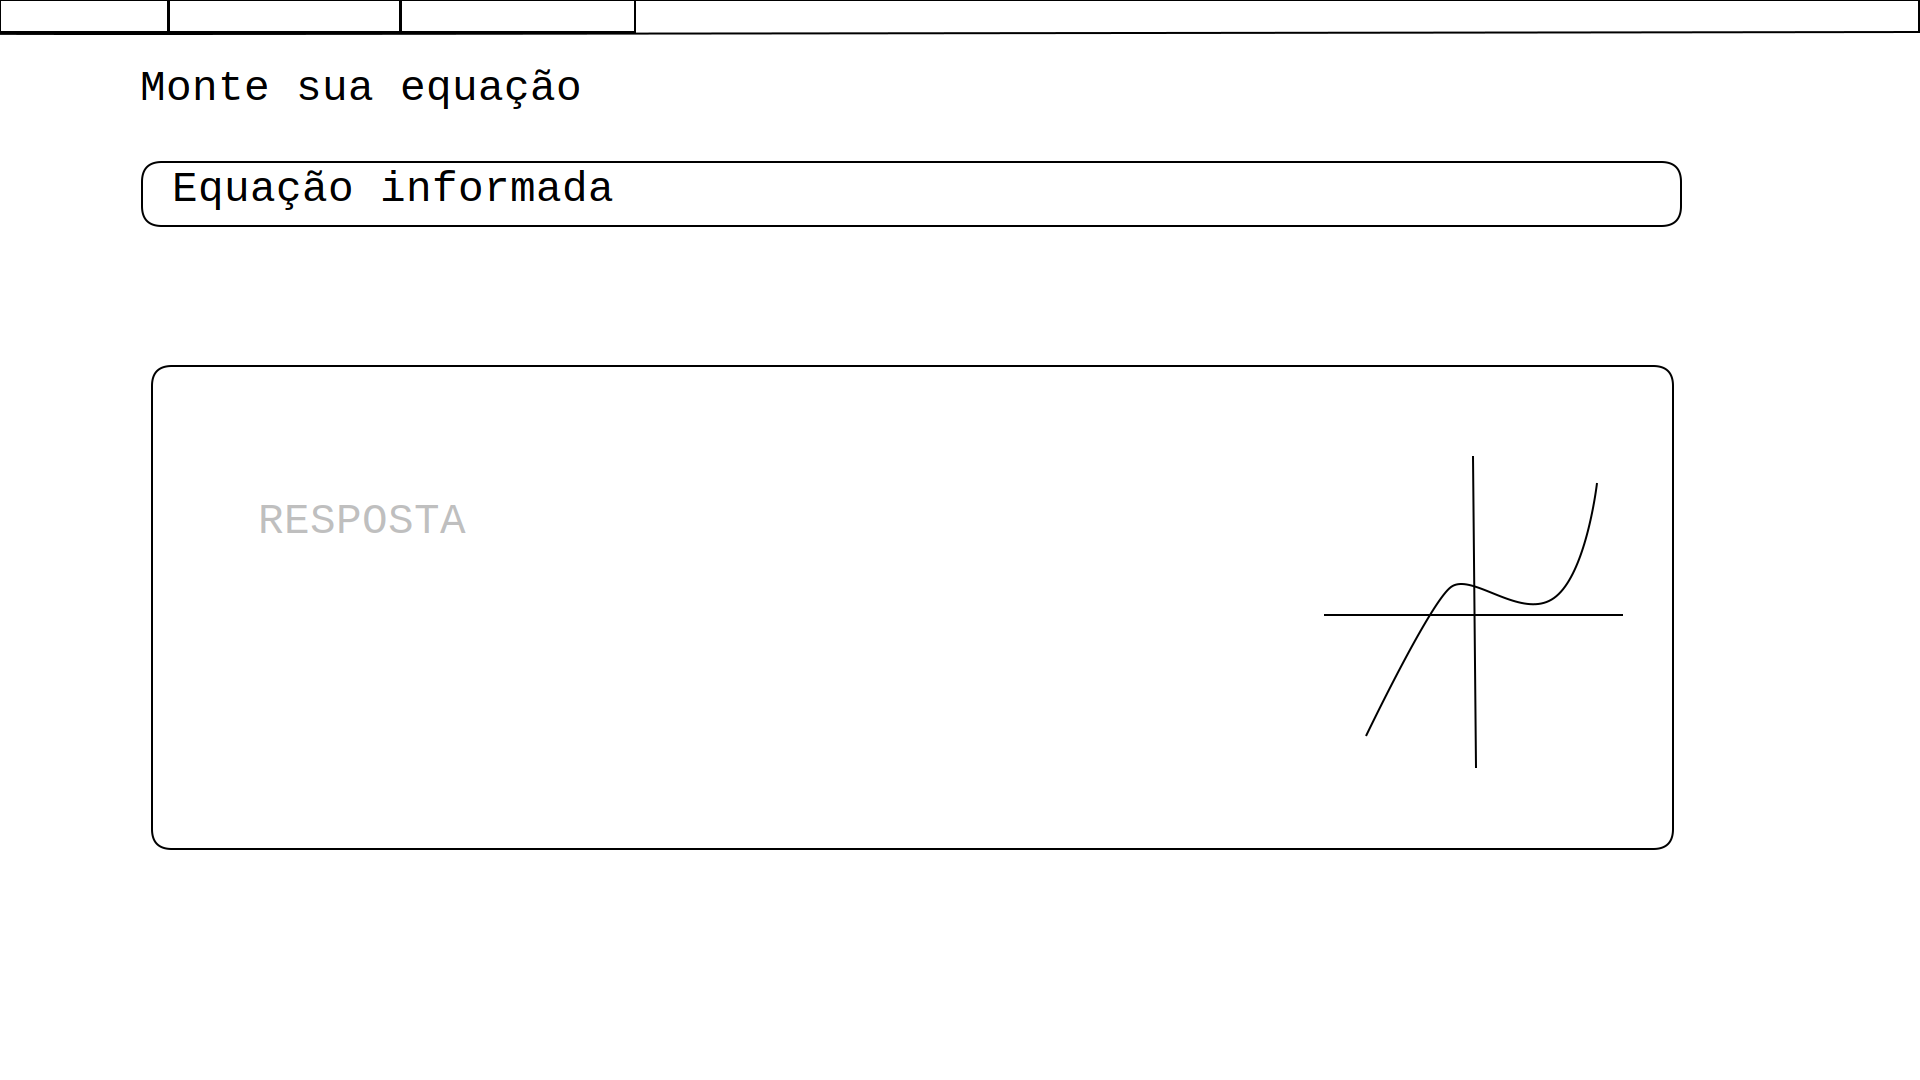
\includegraphics[width=1\textwidth]{img/d.png}
    \caption{Esboço da tela tela de exercícios}
\end{figure}

O portal já está em desenvolvimento e poderá mudar com o tempo e até serem adicionadas novas páginas. O esboço atual é o básico do layout que o projeto seguirá. Para acessar a versão mais recente do portal, pode ser usado o seguinte link: \url{https://pedenite.github.io/PILC-eq/}.

\chapter{Considerações}
Podemos perceber que cada aluno possui sua maneira de estudar e assimilar os conteúdos passados e com o auxílio das ferramentas tecnológicas cada pessoa pode escolher uma que ajude a entender a matéria mais facilmente. O portal em desenvolvimento procura de certa forma, agradar a todo tipo de público, com um visual moderno e a opção de usar temas escuros, tudo para que o usuário sinta-se mais confortavel com a ferramenta, o que é importantíssimo para uma potencialidade no aprendizado.

A interdisciplinaridade, apesar de ainda não incluída no projeto, é um componente importantíssimo do trabalho, que pode ajudar os alunos a compreenderem melhor o conteúdo ao integrá-lo com o mundo real e com outras disciplinas. Serão apresentados conteúdos da física e química para auxiliar no entendimento das equações e da necessidade de seu uso, também podendo auxiliar nas outras disciplinas.

\begin{thebibliography}{9}

\bibitem{Equação do Primeiro Grau}
\noindent Toda Matéria, 
\textit{Equação do Primeiro Grau}
\url{https://www.todamateria.com.br/equacao-do-primeiro-grau/}

\bibitem{Equação do 2° grau}
\noindent Brasil Escola, 
\textit{Equação do 2º grau}
\url{https://brasilescola.uol.com.br/matematica/equacao-2-grau.htm}

\bibitem{Computador na sociendade do conhecimento}
\noindent histórica. In VALENTE, José Armando (org). 
\textit{O computador na sociedade do conhecimento. Campinas: Nied, 2002 Mudanças.}

\bibitem{Interdisciplinaridade: um avanço na educação}
\noindent Meire Cavalcante,
\textit{Interdisciplinaridade: um avanço na educação, 07 de Março de 2018}
\url{https://novaescola.org.br/conteudo/249/interdisciplinaridade-um-avanco-na-educacao?gclid=Cj0KCQjwvvj5BRDkARIsAGD9vlLfazfTkFERfofB1vN-V7rDxoXGWm8athfWhg9VkX2lQnP6Awbh_EsaAnAFEALw_wcB}

\bibitem{Livro interdisciplinaridade}
\noindent Ivani Catarina Arantes Fazenda, Herminia Prado Godoy (2017).
\textit{Interdisciplinaridade: pensar, pesquisar e intervir}

\bibitem{TCC equação do 1 grau}
\noindent José Suelio Lourenço Leite (2019)
\textit{Equações de 1º Grau: A Importância de Práticas Interligadas ao Cotidiano do Aluno}

\end{thebibliography}

\end{document}
